\newpage
\section{Heating Adobe Houses} \label{houses}

Houses in desert climates are usually built using adobe. It is a construction material that uses soil (a mixture of clay, sand and water), stabiliser and binder as raw materials that are mixed and moulded to form sun-dried blocks. Due to this, adobe houses are known for their great thermal efficiency. 

The thicker the adobe walls are, the better, as it will maintain a nearly constant inside temperature. However, it would also be more expensive to build. Here, we try to model the heat flow through adobe walls using the heat equation to find the optimum wall thickness. For this, we use synthetic data, which approximates the typical diurnal temperature variation in these climatic regions.

\subsection{Approximating Temperature Variation}
Desert climates are known for their high variability in temperature throughout the day. For this project, I have used the temperature profile of Sukkur, Rajasthan, which is located around 200 km from the Thar Desert\footnote{Source: \href{https://www.timeanddate.com/weather/@1270835/climate}{timeanddate.com}}. During winters, the temperature can vary from 9 $^\circ$C to 16 $^\circ$C and during summers the variation is from 29 $^\circ$C
to 45 $^\circ$C. An approximate average of this is implemented in the project. 

Using diurnal temperature variations models described in \cite{parra-saldivar-2005}, the external temperature variation can be approximated as a sinusoidal curve, as shown in Fig. \textit{\ref{external_temps}}.

\begin{figure}[H]
    \centering
    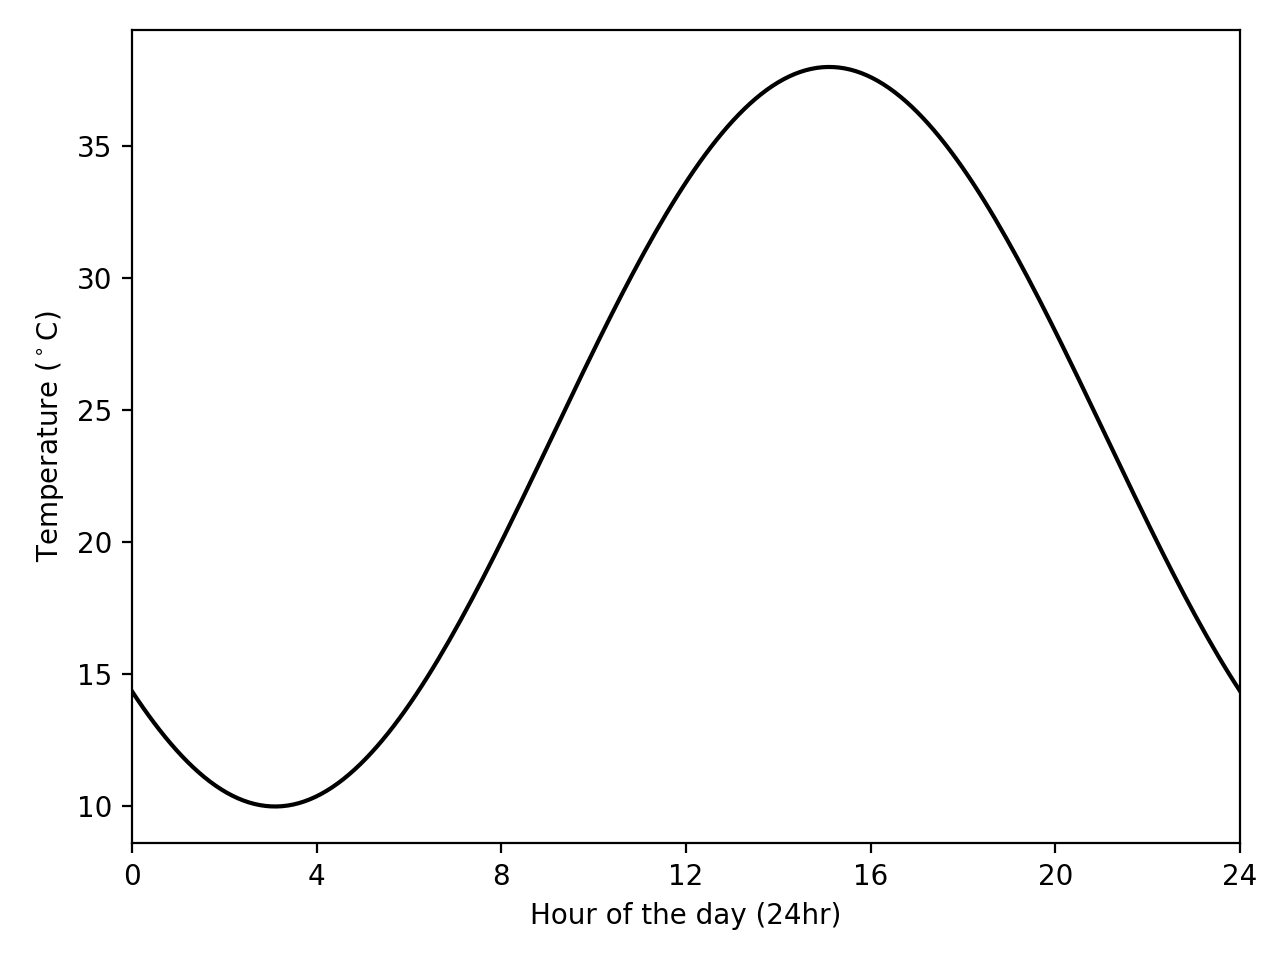
\includegraphics[width=0.6\linewidth]{Figures/4/external.png}
    \caption{Dirunal temperature variation modelled for a day using a sinusoidal curve with equation: $y= 14\sin(\pi x/12 + 3.9) + 24$. The parameters we manually adjusted so that the minimum temperature ($\sim$ 10$^\circ$C) falls around 03:00 and the maximum ($\sim$ 37$^\circ$C) around 15:00 in the day.}
    \label{external_temps}
\end{figure}

% https://www.sciencedirect.com/science/article/abs/pii/S0360132305003082

\subsection{Theoretical Approach}
The heat equation describes the flow of heat through a 3 dimensional space,

\begin{align}
    \frac{\partial T}{\partial t} = \frac{k}{c_p\rho}\left(\frac{\partial^2 T}{\partial x^2} + \frac{\partial^2 T}{\partial y^2} + \frac{\partial^2 T}{\partial z^2}\right)
\end{align}

where $c_p$ is the specific heat of the adobe, $\rho$ is the mass density of the adobe, and $k$ is the thermal conductivity of the adobe. For simplicity we consider $D=\frac{k}{c_p\rho}$, whose standard value is around $0.27$ mm$^2$/s for adobe materials. 

\subsubsection{One Dimensional Case}
Consider a infinitesimally thick rod of length L on which we will numerically solve the heat equation. We can discretise space and time into $\Delta x$ and $\Delta t$ respectively. The left end of the rod ($x=0$) will be our external wall, and hence its temperature will change as a function of time, as discussed in the previous section. The right end ($x=L$) will be the inner wall.

We can use the finite difference method to solve this partial differential equation. This is also called the forward time-centered space (FTCS) method. The iterative finite difference formula for the heat equation (using the approximation for the first and second derivtives) would be:

\begin{align}
   \frac{T_{(t+1,\,x)}-T_{(t,\,x)}}{\Delta t} = D\frac{T_{(t,\,x+1)}-2T_{(t,\,x)}+T_{(t,\,x-1)}}{(\Delta x)^2}
\end{align}

Here we are using the FTCS method because it the least numerically intensive. Also, as the external temperature changes as a function of time, so does our boundary conditions (especially on the left edge). FTCS allows us to have flexible boundary conditions as opposed to other methods like backward difference or the Crank-Nicholson method. 

On the right edge we will assume Neumann boundary conditions $\left(\frac{\partial T}{\partial n} = 0\right)$ as the heat flows into the air inside the house. Mathematically this means $T_{x=N} = T_{x=N-1}$.

\subsubsection{Extension to higher dimensions}
The same finite difference approach can be similarly extended to 2 or 3 dimensions. However here we make a key simplification. Assuming the heat only flows from the external surface to the internal surface and that no significant heat flows into the ground or the roof, we can consider $\frac{\partial T}{\partial z} = 0$. We have reduced the dimension of our problem by 1. 

Now, consider that the wall has a fixed width $W$ and thickness $L$. Here, we assume that the entire external surface is at the same temperature. This is obviously not true since the Sun's inclination throughout the day can lead to non-uniform heating. We also ignore the possibility of windows or other heat outlets from the house. So, if the assumption is true, the heat should spread through the wall uniformly; hence, we can further reduce the dimension of our problem by 1. To put it more precisely, if you assume the wall to be stacked with $N$ layers horizontally, each layer will have the same temperature and no temperature flow will occur within a particular layer (Fig. \ref{layers}).

\begin{figure}[H]
    \centering
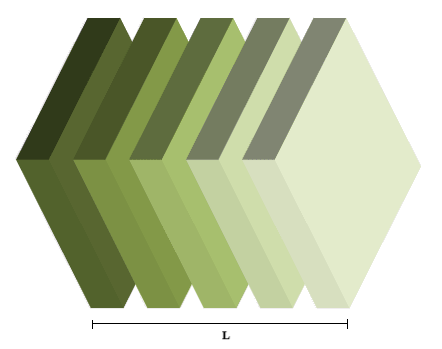
\includegraphics[width=0.6\linewidth]{Figures/4/layers.png}
    \caption{A model of a wall for demonstration, consisting of 5 layers, each with a fixed temperature}
    \label{layers}
\end{figure}

Hence, the optimum thickness obtained from our one-dimensional problem will be, at most, an upper limit if we relax some of the above assumptions (there are more heat sinks to consider). 

\subsection{Implementation}
The following Python code uses the \verb|NUMBA| module, which generates optimized machine code to speed up the computation process.
\begin{lstlisting}[language=Python, caption=Finding the closest possible emission line to match with from the database]
import numpy as np
import matplotlib.pyplot as plt
from numba import jit, cuda

K0 = 273.15 # 0 Celsius in Kelvin

@numba.jit("f8(f8)", nopython=True, nogil=True, fastmath = True)
def external_temperature(sec):
    h = sec/3600
    h = h%24
    t = 15*np.sin(np.pi*h/12 + 3.9) + 24
    return K0 + t

### Defining the problem
alpha = 0.27 # mm^2/sec
days = 7
duration = 3600*24*days #seconds
nodes = 300 # space discretized into nodes 

# initialize wall temperature as a gradient
# where initial inner wall is set at 25 degree Celsius
wall = np.linspace(external_temperature(0), 25+K0, nodes) 

### Solving the heat equation
@numba.jit("(f8[:],f8,f8,f8)", nopython=True, nogil=True, fastmath = True, cache=True)
def solve_heat_eqn(init_state, duration, dt, dx):
    wall = init_state.copy()
    counter = 0
    inners = []
    
    while counter < duration :
        w = wall.copy()
        for i in range(1, nodes - 1):

            wall[i] = dt * alpha * (w[i - 1] - 2 * w[i] + w[i + 1]) / dx ** 2 + w[i]

        counter += dt
        wall[0] = external_temperature(counter)
        wall[-1] = wall[-2] # Neumann BC
        
        inners.append(wall[-1])
        
    return wall, np.array(inners)

# Solve heat equation for a particular wall thickness
def get_inner_temperatures(thickness):
    dx = thickness / (nodes-1)
    dt = 0.5 * dx**2 / alpha
    final, inners = solve_heat_eqn(wall, duration, dt, dx)
    return inners   

variations = {}

# plotting $\Delta T$ vs thickness.
thicknesses = [T for T in range(170, 300, 10)]
for thickness in thicknesses:
    inner_temps = get_inner_temperatures(thickness)
    stable_region = int(len(inner_temps)/2)
    maxT = np.max(inner_temps[stable_region:])
    minT = np.min(inner_temps[stable_region:])
    variations[thickness] = maxT-minT

plt.figure(figsize=(9,7))
variations = dict(sorted(variations.items()))
plt.plot(variations.keys(), variations.values(), '-ko')
plt.ylabel(r'$\Delta T$ ($^\circ$C)')
plt.xlabel('Thickness (mm)')
\end{lstlisting}

\subsection{Results}
\begin{figure}[H]
    \centering
    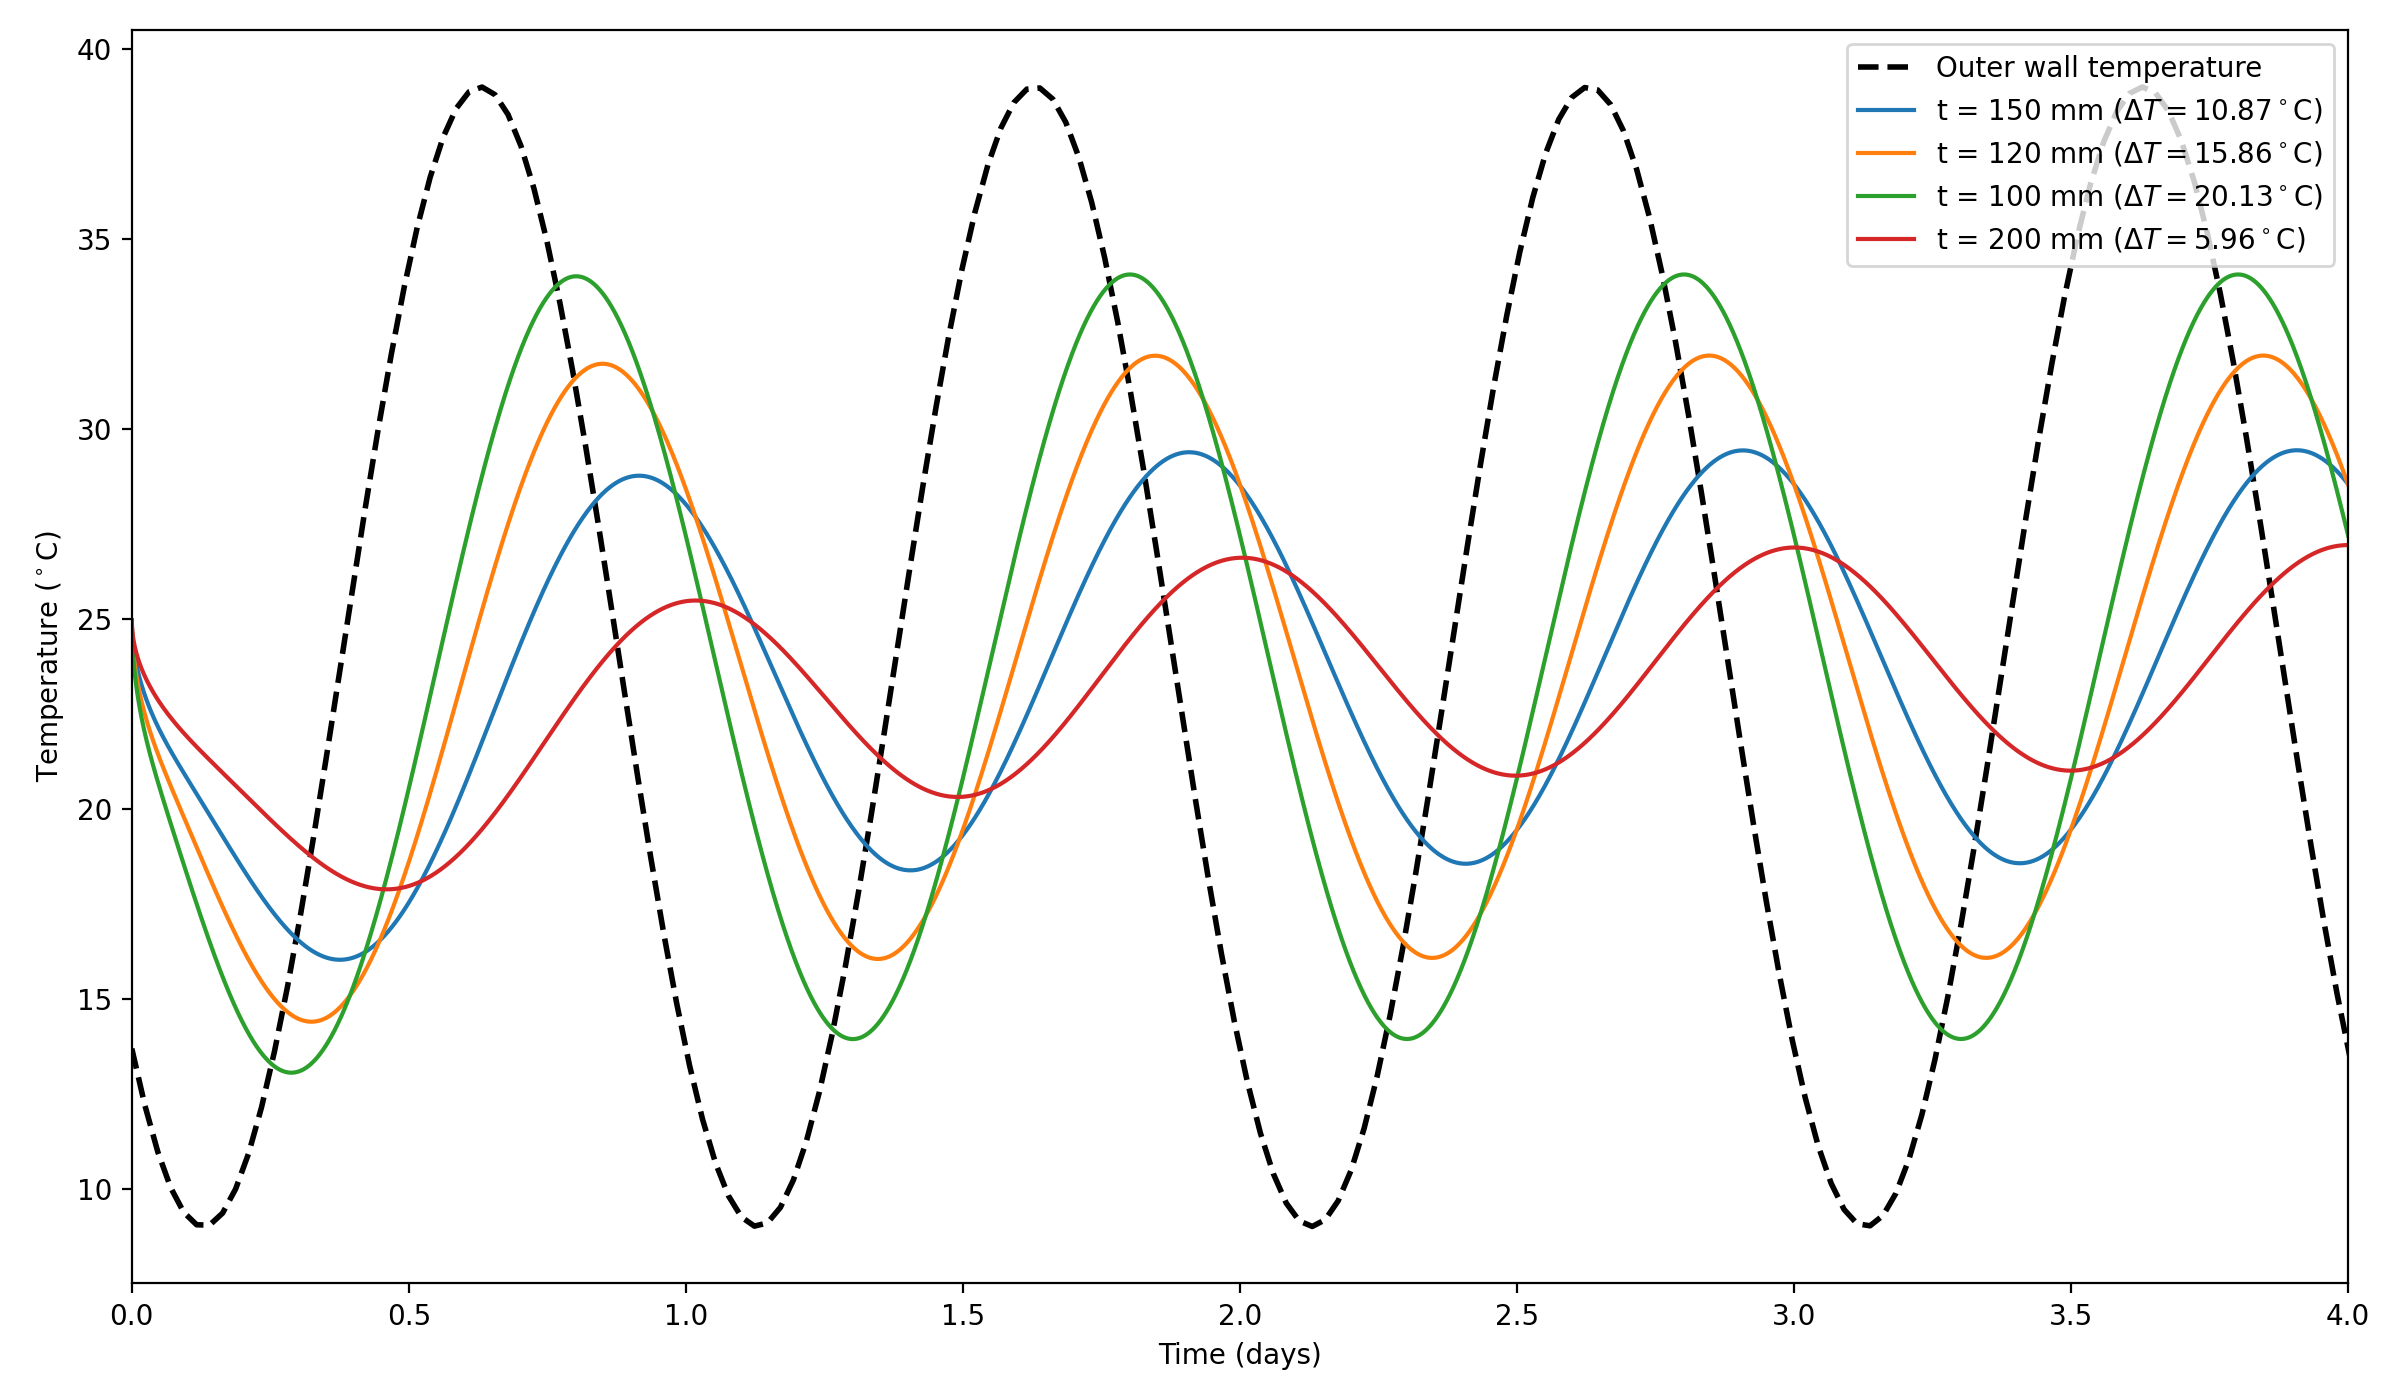
\includegraphics[width=0.7\linewidth]{Figures/4/var0.png}
    \caption{The inside temperature for different wall thicknesses compared to outside temperature. Note that as the thickness increases, not only does the temperature variation inside decrease, but also the time taken for the outside conditions to affect the inside of the wall increases.}
    \label{var0}
\end{figure}

The above two plots show the temperature of the inner wall as a function of time, with the temperature of the outer wall for comparison. We have given a few days to simulate the temperature variations to achieve a steady state. 
\begin{figure}[H]
    \centering
    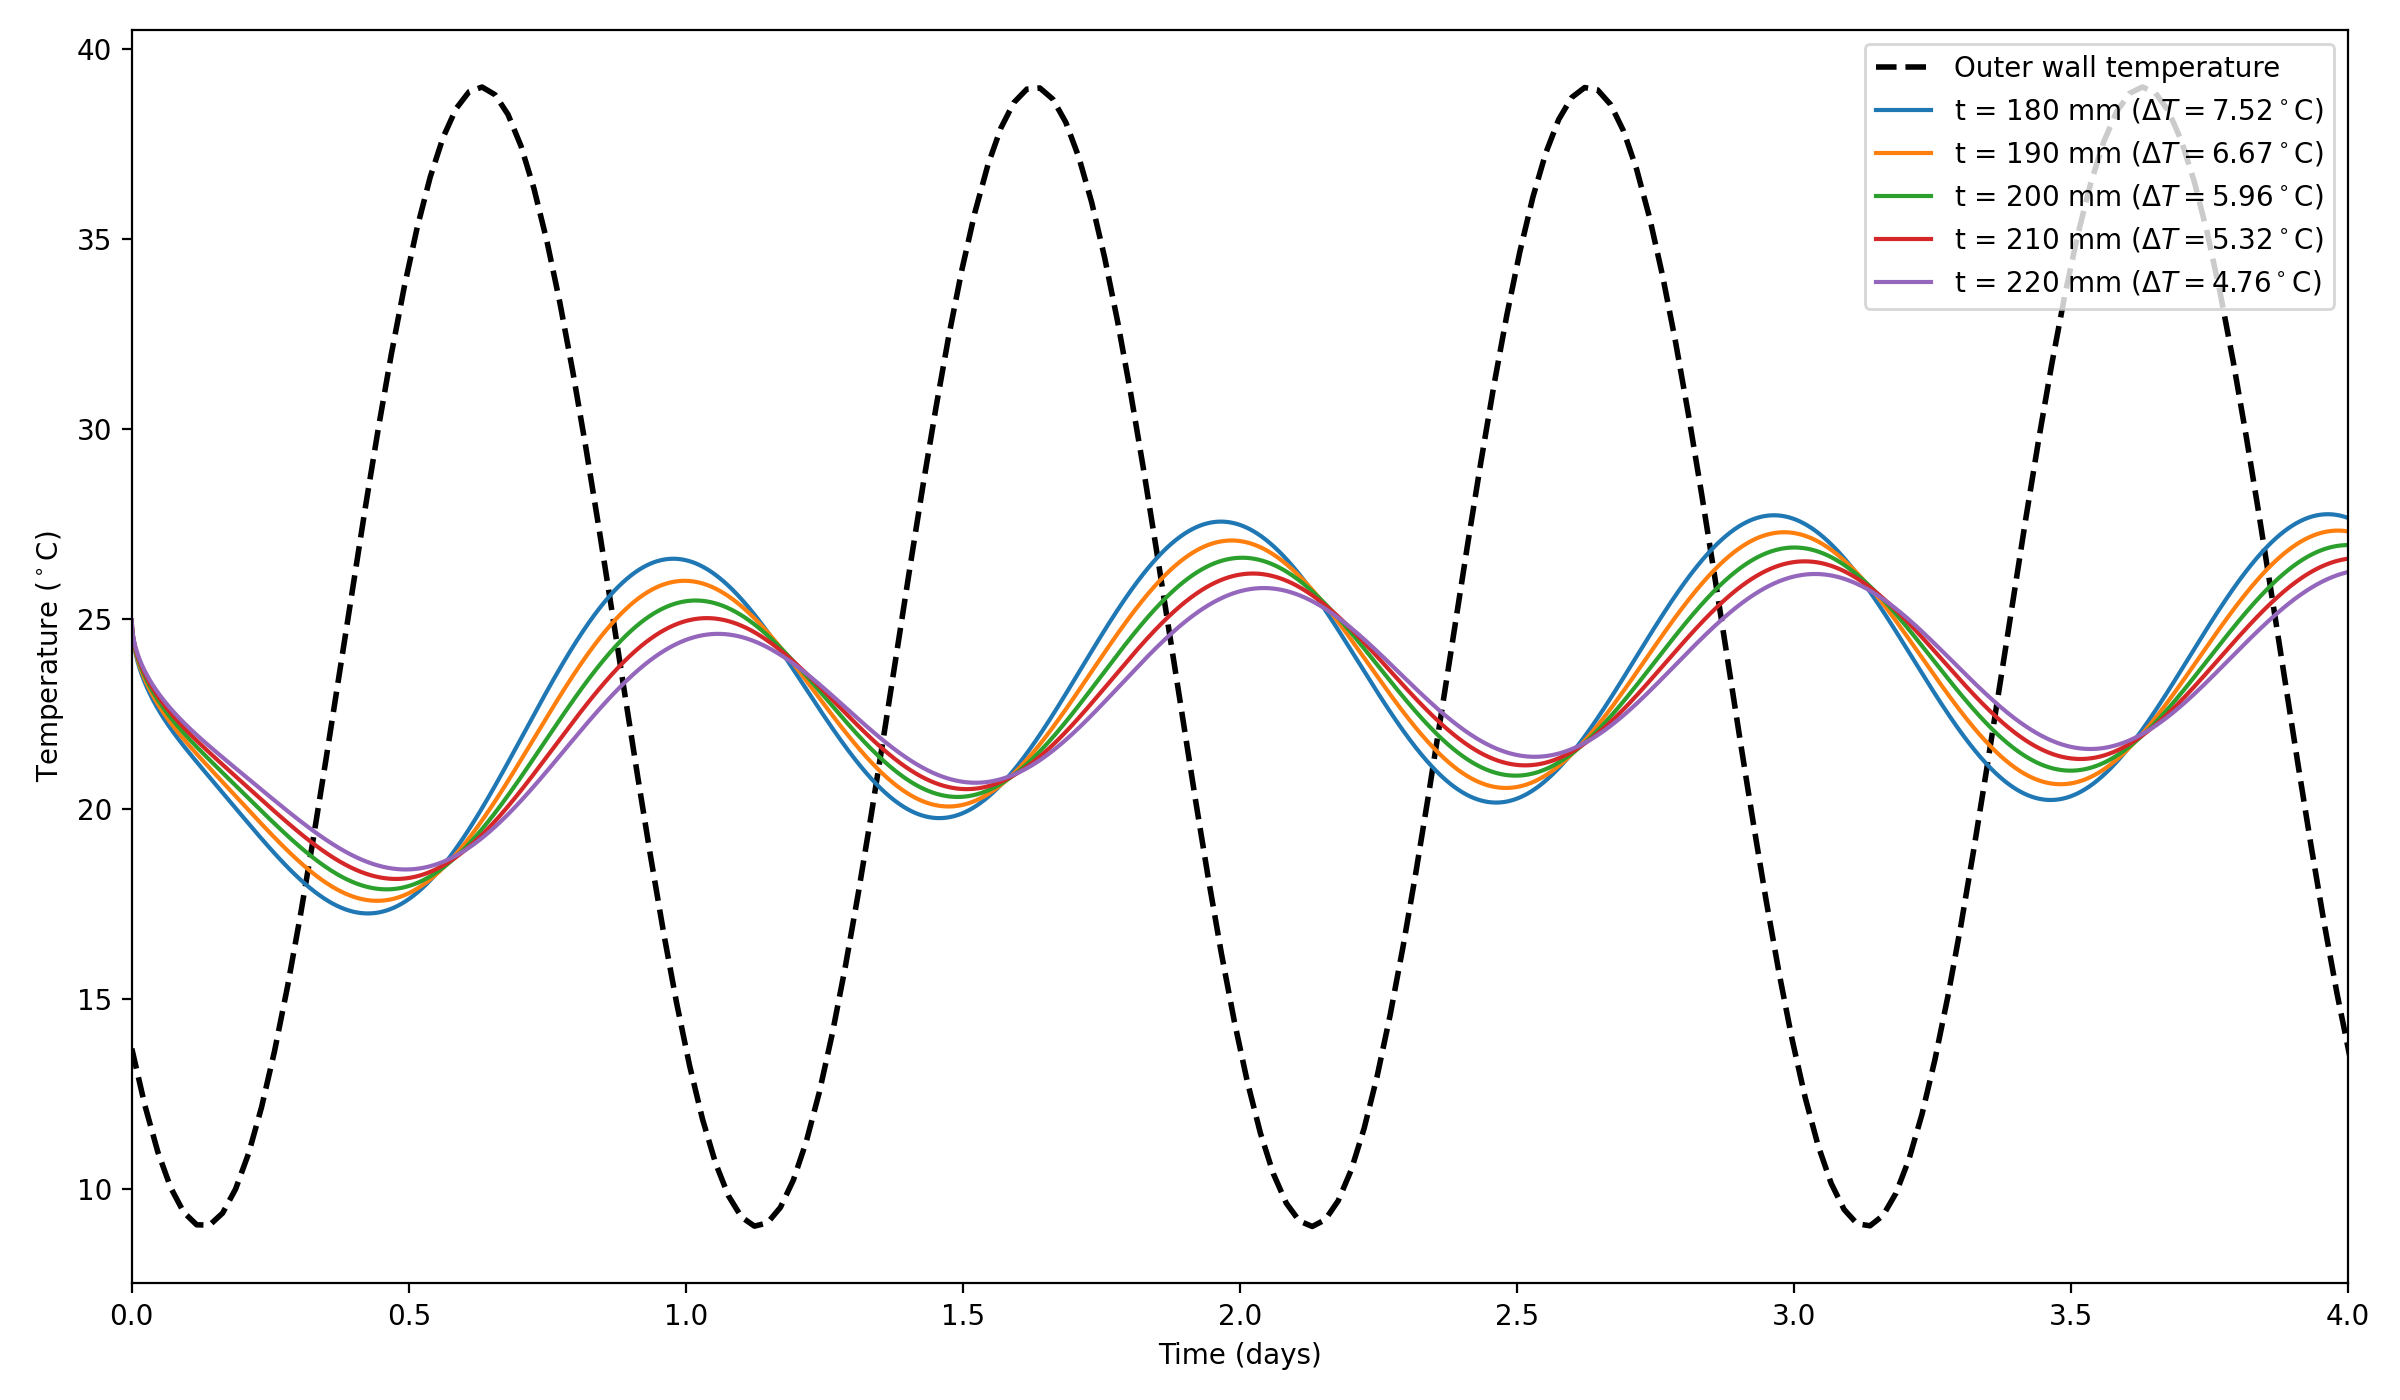
\includegraphics[width=0.7\linewidth]{Figures/4/var1.png}
    \caption{Similar to the above plot but for a higher value of wall thicknesses. The temperature variation becomes less and less extreme as the thickness increases.}
    \label{var2}
\end{figure}

% \begin{figure}[H]
%     \centering
%     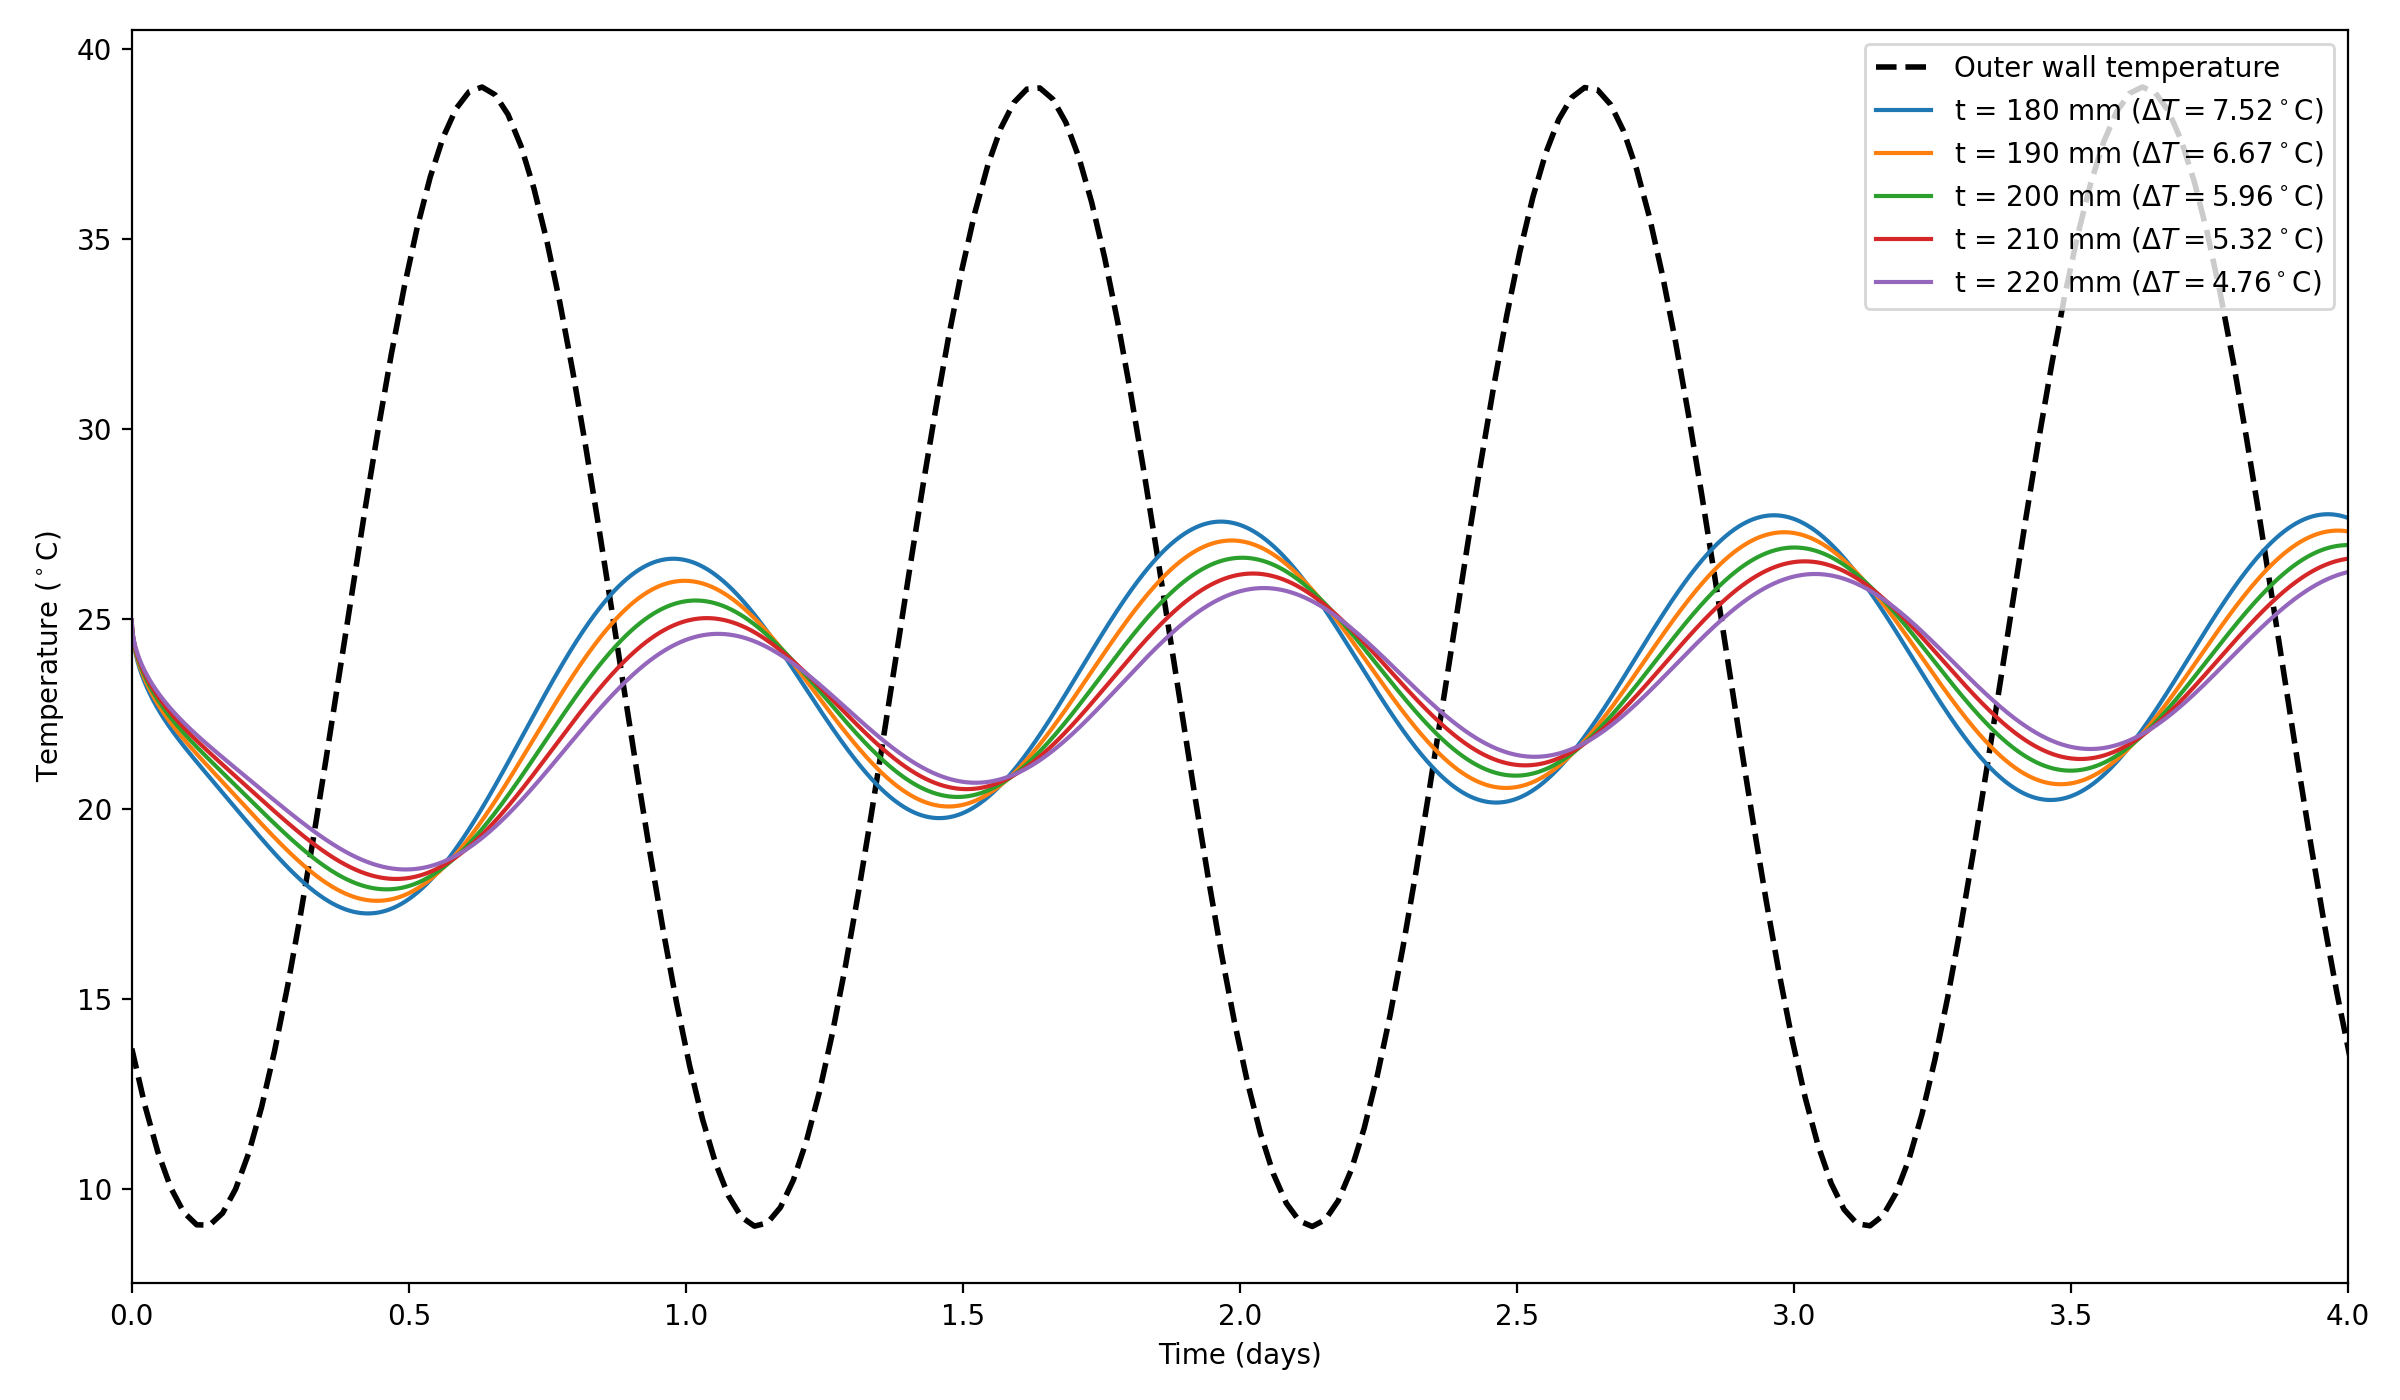
\includegraphics[width=0.7\linewidth]{Figures/4/var1.png}
%     \caption{}
%     \label{var1}
% \end{figure}
Fig. \ref{var_fin} shows the temperature variation, $\Delta T$, as a function of wall thickness. We can see the variation is not linear and slows down particularly after $\sim$ 200 mm (for Adobe).  

\begin{figure}[H]
    \centering
    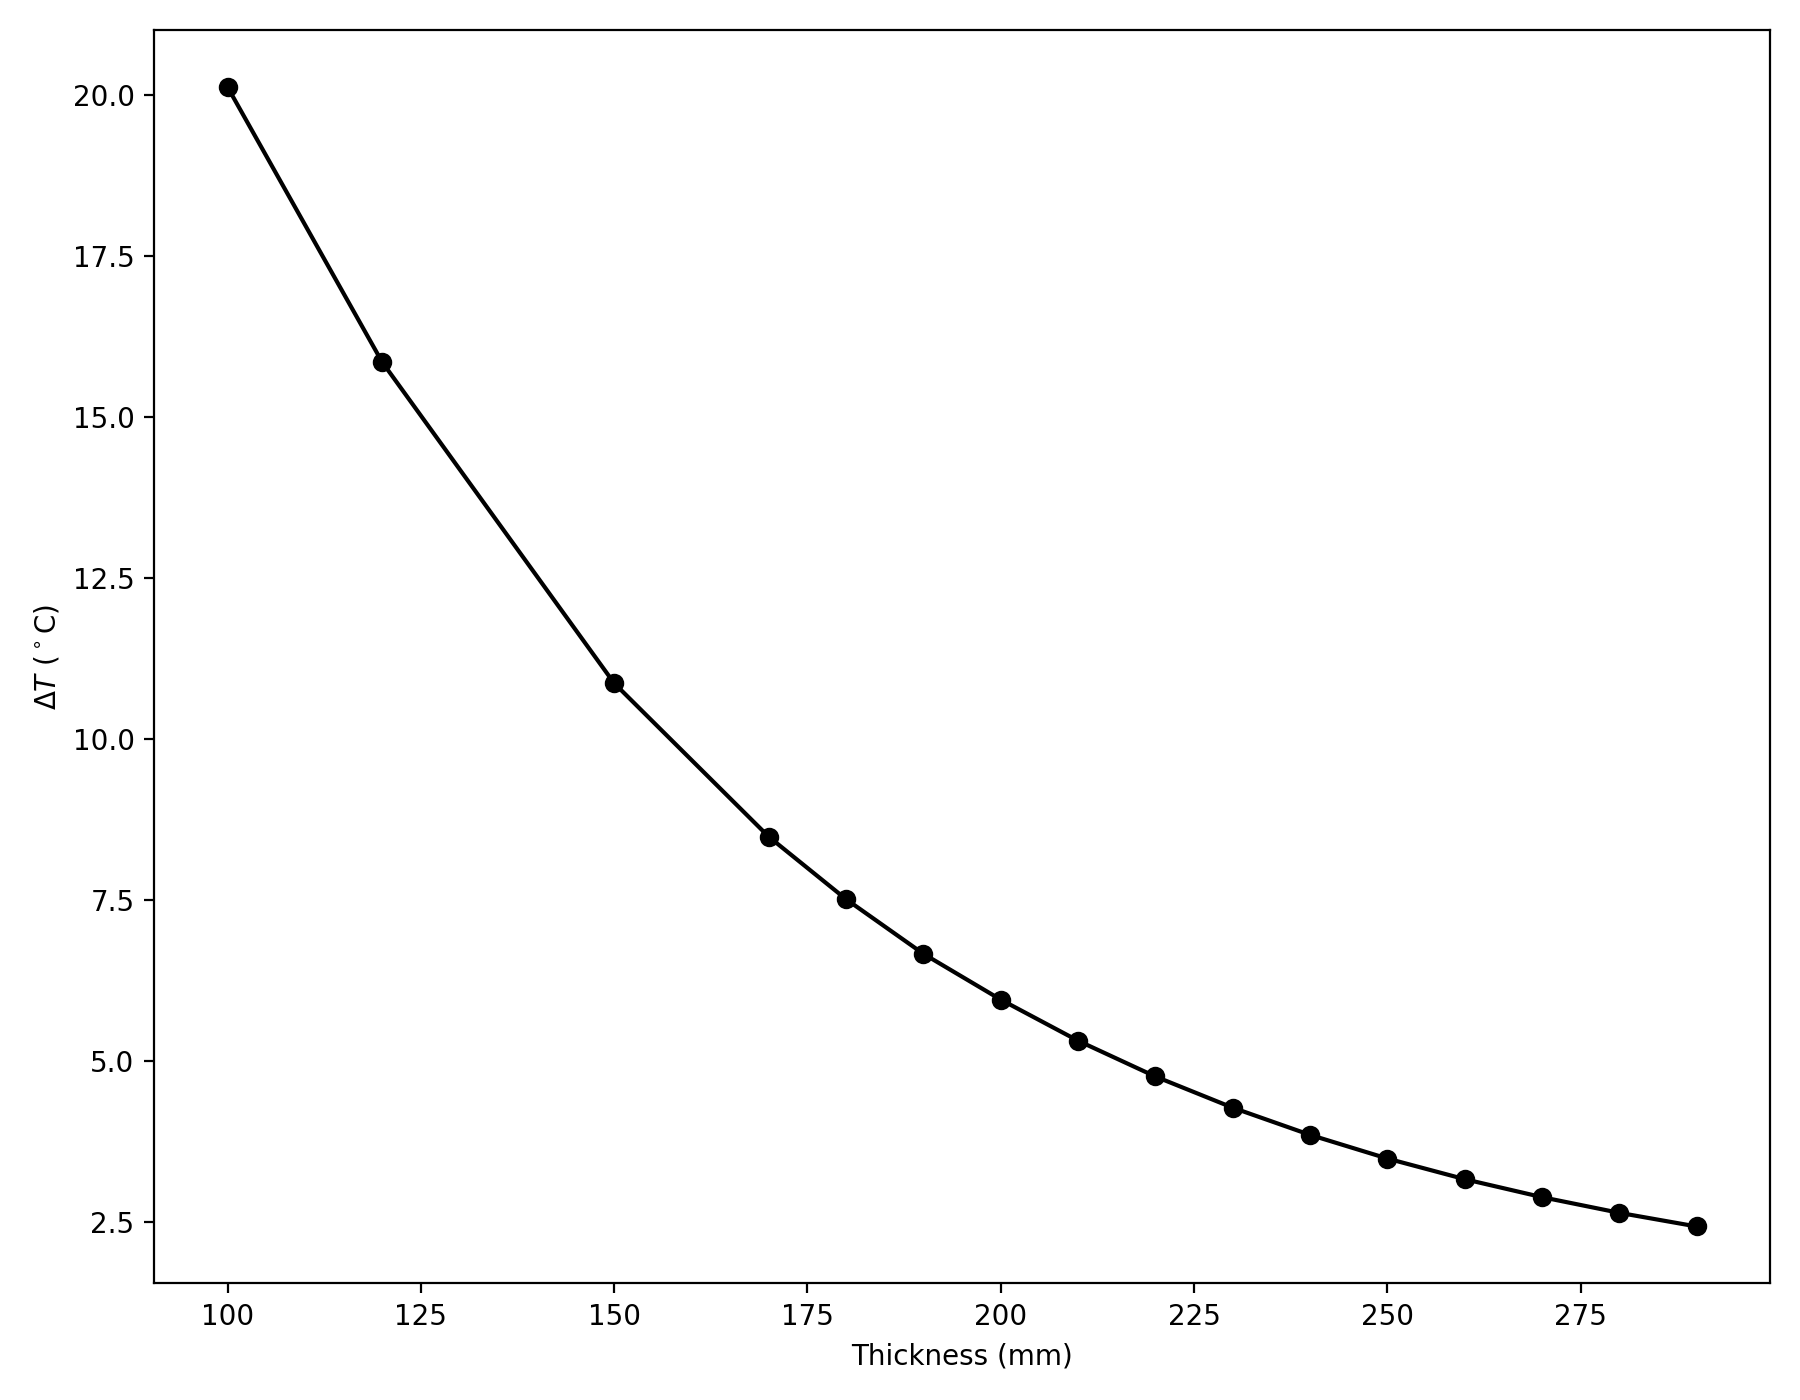
\includegraphics[width=0.6\linewidth]{Figures/4/var_fin.png}
    \caption{Final temperature variation $\Delta T$ vs  wall thickness plot}
    \label{var_fin}
\end{figure}

\subsection{Discussion}
According to \cite{public-health-england-2013}, the comfortable range of temperature variation for human beings is around 3 to 4 $^\circ$C (more precisely 20 to 24 $^\circ$C). From Fig. \ref{var_fin}, we can see that the temperature variations are in the comfortable range for wall thicknesses $\ge$ 220mm. So, to minimise the construction cost, 220mm would be the ideal wall thickness. 

Due to the simplifications we made along the way, including reducing the dimensions by 2 and assuming uniform heating mean that the obtained value would be the minimum wall thickness required for adobe walls to remain at a comfortable temperature. Hence, this result broadly agrees with the values argued by \cite{parra-saldivar-2005}, which are $\sim$ 340mm. (Note that the paper also takes into account multilayer walls and walls with windows). 